
\section{Implementacija}

Razvijeni model optimizacije implementiran je u programskom jeziku \textbf{Python (verzija 3.x)}, odabranom zbog čitljivosti, bogatog ekosustava biblioteka i široke primjene u znanstvenom računarstvu \cite{PythonSoftwareFoundation}. Python omogućuje brzu izradu prototipa, jednostavnu integraciju modula te učinkovitu obradu i vizualizaciju podataka.

\subsection{Korištene biblioteke}

Za izradu sustava korištene su sljedeće biblioteke (Tablica~\ref{tab:biblioteke}):

\begin{table}[H]
\centering
\caption{Korištene biblioteke u implementaciji}
\label{tab:biblioteke}
\begin{tabular}{|l|p{10cm}|}
\hline
\textbf{Biblioteka} & \textbf{Namjena i citat} \\ \hline
Python & Osnovni programski jezik za cjelokupnu implementaciju. \cite{PythonSoftwareFoundation} \\ \hline
DEAP & Okvir za razvoj i provedbu evolucijskih algoritama. \cite{DEAP2012} \\ \hline
NumPy & Numeričke operacije i statistička obrada nizova podataka. \cite{Harris2020} \\ \hline
Pandas & Učitavanje, obrada i spremanje tabličnih podataka s rezultatima. \cite{PandasDevelopmentTeam2020} \\ \hline
Seaborn & Kreiranje naprednih statističkih vizualizacija (stupčasti, linijski i raspršeni grafikoni). \cite{Waskom2021} \\ \hline
Matplotlib & Osnovna biblioteka za crtanje na koju se oslanja Seaborn. \cite{Hunter2007} \\ \hline
Random & Standardna Python biblioteka korištena za generiranje slučajnih brojeva i uzorkovanje iz Trokutaste distribucije. \\ \hline
\end{tabular}
\end{table}
\subsection{Struktura sustava}


Sustav razvijen za potrebe ovog rada predstavlja cjeloviti eksperimentalni okvir dizajniran za analizu, kalibraciju i usporedbu optimizacijskih metodologija. Umjesto jednostavnog, monolitnog sustava, arhitektura je modularna i sastoji se od dva glavna analitička modula te jednog pomoćnog modula za obradu rezultata:

\begin{enumerate}
    \item \textbf{Modul za analizu i kalibraciju genetskog algoritma} \\
    Ovaj modul predstavlja temelj istraživanja i odgovara na pitanje: \emph{``Kako optimalno konfigurirati genetski algoritam za rješavanje zadanog problema?''}. Njegova primarna svrha je provođenje detaljne ablacijske studije (Ablation Study) kako bi se ispitao utjecaj svakog ključnog parametra na performanse algoritma.
    
    \textbf{Funkcionalnosti:}
    \begin{itemize}
        \item Sustavno testiranje različitih konfiguracija genetskog algoritma (standardni GA, bez križanja, bez mutacije, s povećanim brojem generacija, s većom populacijom).
        \item Višestruko pokretanje (\( \text{RUNS} = 10 \)) svake konfiguracije radi osiguravanja statističke značajnosti rezultata.
        \item Izračunavanje metrika performansi, uključujući prosječnu vrijednost (mean) i standardnu devijaciju (std) za ROI i procijenjeno trajanje.
        \item \textbf{Izlaz modula:} ``Šampionska'' konfiguracija – skup optimalnih parametara za genetski algoritam koji će se koristiti u daljnjoj analizi.
    \end{itemize}

    \item \textbf{Modul za usporednu analizu optimizacijskih scenarija} \\
    Ovaj modul čini srž diplomskog rada i koristi ``šampionsku'' konfiguraciju, definiranu u prethodnom modulu, za provođenje konačne usporedbe triju različitih pristupa rješavanju problema.
    
    \textbf{Funkcionalnosti:}
    \begin{itemize}
        \item Implementacija i izvršavanje triju ključnih scenarija:
        \begin{itemize}
            \item \textbf{Osnovni model (Random Search):} Slučajan odabir kao temeljna linija za usporedbu.
            \item \textbf{Klasični genetski algoritam:} Optimizacija usmjerena isključivo na maksimizaciju ROI-a.
            \item \textbf{Hibridni GA+MC model (NSGA-II):} Više-objektivna optimizacija koja istovremeno maksimizira ROI i minimizira rizik trajanja procijenjen Monte Carlo simulacijom.
        \end{itemize}
        \item Statistički robusna usporedba temeljem višestrukih pokretanja (\( \text{RUNS} = 10 \)) svakog scenarija.
        \item \textbf{Ulaz modula:} Optimalni parametri genetskog algoritma dobiveni iz Modula~1.
        \item \textbf{Izlaz modula:} Konačna tablica s usporednim rezultatima performansi (ROI, trajanje) i stabilnosti (standardna devijacija) za svaki od triju scenarija.
    \end{itemize}

    \item \textbf{Modul za obradu i vizualizaciju rezultata} \\
    Ovaj modul nije sekvencijalni korak, već pomoćni alat koji služi za interpretaciju rezultata dobivenih iz prva dva modula.
    
    \textbf{Funkcionalnosti:}
    \begin{itemize}
        \item Generiranje preglednih tablica s rezultatima pomoću \texttt{pandas} biblioteke.
        \item Spremanje rezultata u CSV format za daljnju analizu i dokumentaciju.
        \item (Potencijalno) stvaranje grafičkih prikaza, kao što su stupčasti dijagrami za usporedbu prosječnih vrijednosti ili 2D raspršeni dijagrami (scatter plots) za prikaz Paretovog fronta dobivenog iz NSGA-II algoritma.
    \end{itemize}
\end{enumerate}

\begin{figure}[H]
    \centering
    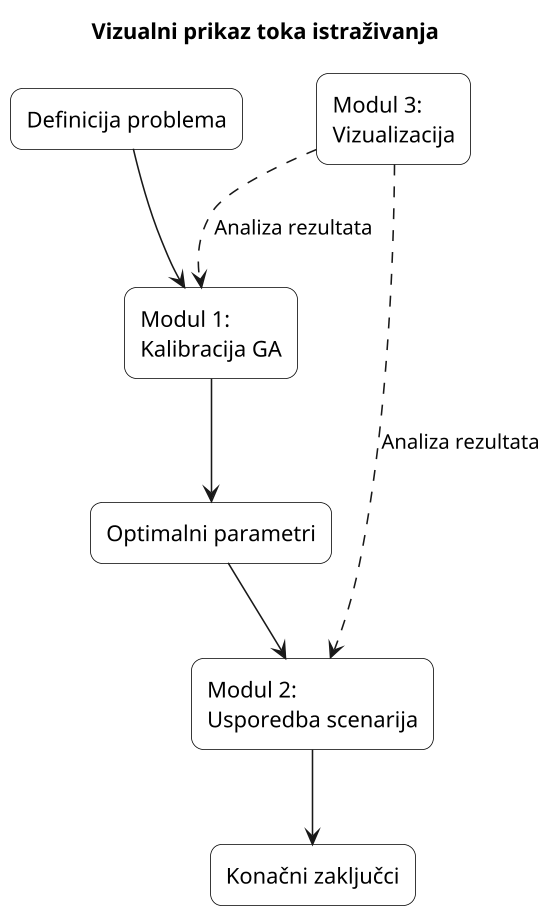
\includegraphics[width=0.9\textwidth]{slike/tijek_istrazivanja.png}
    \caption{Vizualni prikaz toka istraživanja}
    \label{tok istraživanja}
\end{figure}

\subsection{Modeliranje nesigurnosti: Monte Carlo simulacija}

Za svaku projektnu aktivnost definirane su tri točke procjene trajanja:
\[
a \ (\text{optimistična}), \quad
m \ (\text{najvjerojatnija}), \quad
b \ (\text{pesimistična})
\]
Iako u teoriji postoje kompleksnije distribucije poput \textit{Beta-PERT} distribucije, 
za potrebe ovog rada odabrana je \textbf{Trokutasta distribucija (Triangular distribution)} 
zbog svoje praktičnosti, računalne efikasnosti i intuitivnog temelja na tri poznate procjene.

\paragraph{Generiranje trajanja aktivnosti.}
U svakoj iteraciji Monte Carlo simulacije, trajanje svake aktivnosti generira se slučajnom vrijednošću 
unutar raspona $[a, b]$ s najvećom vjerojatnošću u točki $m$.  
Trokutasta distribucija definirana je funkcijom gustoće vjerojatnosti:
\[
f(x) =
\begin{cases}
\frac{2(x-a)}{(b-a)(m-a)}, & a \leq x < m, \\
\frac{2(b-x)}{(b-a)(b-m)}, & m \leq x \leq b, \\
0, & \text{inače}.
\end{cases}
\]

\paragraph{Procjena trajanja portfelja.}
Ukupno trajanje projektnog portfelja u jednoj simulaciji dobiva se zbrojem trajanja svih aktivnosti odabranih u tom portfelju:
\[
T_{\text{portfolio}} = \sum_{i \in S} t_i
\]
gdje je $S$ skup odabranih aktivnosti, a $t_i$ generirano trajanje aktivnosti $i$.

\paragraph{Agregiranje rezultata.}
Monte Carlo simulacija ponavlja se velik broj puta $(\text{NUM\_SIMULATIONS})$, a konačna procjena trajanja portfelja 
dobiva se kao prosječna vrijednost svih simuliranih trajanja:
\[
\overline{T}(S) = \frac{1}{\text{NUM\_SIMULATIONS}} \sum_{k=1}^{\text{NUM\_SIMULATIONS}} T_{\text{portfolio}}^{(k)}
\]
gdje $T_{\text{portfolio}}^{(k)}$ označava ukupno trajanje portfelja u $k$-toj simulaciji.

\subsection{Optimizacijski pristup: Genetski algoritam}

Implementacija genetskog algoritma provedena je pomoću programske biblioteke \texttt{DEAP} (Distributed Evolutionary Algorithms in Python) \cite{DEAP2012}. 
S obzirom na prirodu problema odabira podskupa aktivnosti, korištena je \textbf{binarna reprezentacija}.

\paragraph{Reprezentacija jedinke.}
Svaka jedinka (kromosom) u populaciji predstavlja jedno potencijalno rješenje – jedan portfelj projekata. 
Predstavljena je kao binarni niz duljine jednake ukupnom broju aktivnosti $(\text{NUM\_ACTIVITIES})$, gdje gen na poziciji $i$ ima vrijednost:
\[
g_i =
\begin{cases}
1, & \text{ako je $i$-ta aktivnost odabrana}, \\
0, & \text{ako nije odabrana}.
\end{cases}
\]

\paragraph{Funkcija pogodnosti (Fitness Function).}
Ovisno o eksperimentalnom scenariju, korištene su dvije vrste funkcije pogodnosti:

\begin{enumerate}
    \item \textbf{Jedno-kriterijska optimizacija.}  
Za scenarij GA (samo ROI), cilj je bio isključivo maksimizacija ukupnog povrata na investiciju (ROI). Za rukovanje ograničenjem budžeta primijenjena je stroga kaznena metoda. Ako ukupni trošak odabranog portfelja $S$ ne prelazi budžet, njegova pogodnost je jednaka ukupnom ROI-u. U suprotnom, pogodnost postaje negativna vrijednost proporcionalna iznosu prekoračenja:
$$
\text{Fitness}(S) = 
\begin{cases}
    \sum_{i \in S} \text{ROI}_i, & \text{ako } \sum_{i \in S} \text{Trošak}_i \leq \text{Budžet} \\
    -\left(\sum_{i \in S} \text{Trošak}_i - \text{Budžet}\right), & \text{ako } \sum_{i \in S} \text{Trošak}_i > \text{Budžet}
\end{cases}
$$
Ovakav pristup osigurava da svako valjano rješenje (koje ima pozitivan fitness) uvijek bude ocijenjeno kao bolje od bilo kojeg nevaljanog rješenja (koje ima negativan fitness).    \item \textbf{Više-kriterijska optimizacija.}  
    Za hibridni scenarij \texttt{GA+MC} korišten je napredni algoritam NSGA-II, s ciljem istovremene optimizacije dva suprotstavljena kriterija:
    \begin{enumerate}
        \item maksimizirati ROI,
        \item minimizirati prosječno trajanje projekta, procijenjeno Monte Carlo simulacijom.
    \end{enumerate}
    Formalno:
    \[
    \begin{cases}
    \max f_1(S) = ROI(S) \\
    \min f_2(S) = \overline{T}(S)
    \end{cases}
    \]
    gdje $\overline{T}(S)$ označava prosječno trajanje portfelja $S$.
\end{enumerate}

\paragraph{Genetski operatori.}
Za evoluciju populacije korišteni su sljedeći standardni operatori za binarnu reprezentaciju:

\begin{itemize}
    \item \textbf{Selekcija:}  
    Turnirska selekcija (\texttt{tools.selTournament}) za jedno-kriterijsku optimizaciju,  
    te \texttt{tools.selNSGA2} za više-kriterijsku optimizaciju.
    
    \item \textbf{Križanje:}  
    Križanje u dvije točke (\texttt{tools.cxTwoPoint}), koje razmjenjuje segmente između dva roditeljska kromosoma.
    
    \item \textbf{Mutacija:}  
    Slučajna promjena bita (\texttt{tools.mutFlipBit}), koja s malom vjerojatnošću mijenja vrijednost pojedinog gena (iz $0$ u $1$ ili obrnuto), osiguravajući genetsku raznolikost i sprječavajući preranu konvergenciju.
\end{itemize}


\subsection{Vizualizacija}

Za analizu i prikaz rezultata dobivenih optimizacijom korištene su biblioteke \texttt{pandas} za tabličnu obradu podataka te \texttt{}Seaborn} i \texttt{}Matplotlib} \cite{Waskom2021, Hunter2007} za grafičku vizualizaciju.
Kombinacija ovih alata omogućila je jasnu i preglednu prezentaciju rezultata 
dobivenih iz eksperimentalnih scenarija.

Ključni vizualni elementi korišteni u ovom radu uključuju:

\begin{itemize}
    \item \textbf{Tablični prikazi:} Detaljne tablice s konačnim, statistički obrađenim rezultatima 
    usporedbe različitih optimizacijskih scenarija, uključujući osnovne metrike 
    poput prosječnog ROI-a, prosječnog trajanja te raspona vrijednosti.

    \item \textbf{Stupčasti dijagrami:} Koristili su se za vizualnu usporedbu prosječnih vrijednosti 
    (\textit{ROI} i trajanje) između različitih metodologija optimizacije, omogućujući brzu identifikaciju 
    učinkovitijih pristupa.

    \item \textbf{Raspršeni dijagram (Scatter Plot):} Prikaz Paretovog fronta dobivenog NSGA-II algoritmom, 
    koji jasno ilustrira kompromis (\textit{trade-off}) između dvaju suprotstavljenih ciljeva:
    maksimizacije ROI-a i minimizacije trajanja. Time se omogućuje intuitivna procjena 
    učinkovitosti rješenja.
\end{itemize}

Vizualizacija rezultata odigrala je ključnu ulogu u interpretaciji dobivenih podataka, 
posebno u scenarijima s više ciljeva, gdje tablični prikazi sami po sebi nisu dovoljni 
za uočavanje odnosa i kompromisa među varijablama.

